\chapter{Resume (en Francais)}
\label{chapter:resume}
\pagestyle{mainmatter}
\pagenumbering{arabic}

Understanding the human brain is one of the most significant challenges of the 21st century. The human brain is arguably the most complex  organs of the human body, which performs a wide range of cognitive functions: from visual recognition to language understanding, speech, social interaction, and executive control. Pathologies of the brain are perhaps one of the biggest challenges for medicine today. Medical interventions and drugs for major infectious diseases are available today, and individuals can expect to live up to the mid 80s and even into their 90s. Yet, we still do not have a good grasp over most mental pathologies: Parkinson's, Alzheimer's, dementia, epilepsy to name a few. This is despite the fact that someone today who lives into their mid 80s has a 50\% chance of contracting Alzheimer's~\citep{alzheimer20162016}.

Our current understanding of the brain is a result of decades of concerted efforts across multiple disciplines ranging from molecular biology, genetics, physiology, cognitive and behavioral neuroscience, to statistics, computer science, and data science. A relatively new subfield here is brain imaging, also known as neuroimaging. Brain imaging refer to a set of technologies where  snapshots of the brain are taken. These snapshots can be static, as in the case of anatomical images from \ac{MRI}, or an evolving image, as in the case of \ac{fMRI}. The grand vision is to utilize them in hospitals to help diagnosis, in surgeries, in \acp{BCI}, or in research for neuroscientists to better understand the brain. 
In this thesis, we will focus our attention on measuring the electric currents and/or corresponding magnetic field from the brain, using electroencephalography, magnetoencephalography, and local field potentials. 
These methods have the property of possessing a high temporal resolution, which is particularly useful for extracting the temporal dynamics of brain signals.

In this manuscript, I will describe several methodological advances that we achieved in brain imaging using our expertise in machine learning and open source software. In the forthcoming sections, I will first describe the context of the thesis. After a brief introduction to electrophysiology, I will delve into how the field has been shaped in recent years by the reproducibility crisis, and how data sharing is going to help alleviate this problem to a large extent. However, the rise of data sharing and large sample sizes makes it difficult to still rely on manual data analysis which does not scale and is not reproducible. To cope with this challenge, we must start relying on automated and data-driven methods for discovering new effects. To this end, I will introduce two new algorithms \emph{autoreject} and \emph{alphacsc}. This is followed by a refresher on background material that might be useful to refer to when reading the thesis. The chapter ends with the contributions of this thesis and the list of papers published during the PhD.
 
%\section{Modern brain imaging}
%Brain imaging tools today can be placed along three axes: their temporal resolution, their spatial resolution, and the level to which they are invasive.

\section{Electrophysiology}

\begin{figure}[htb]
\begin{center}
   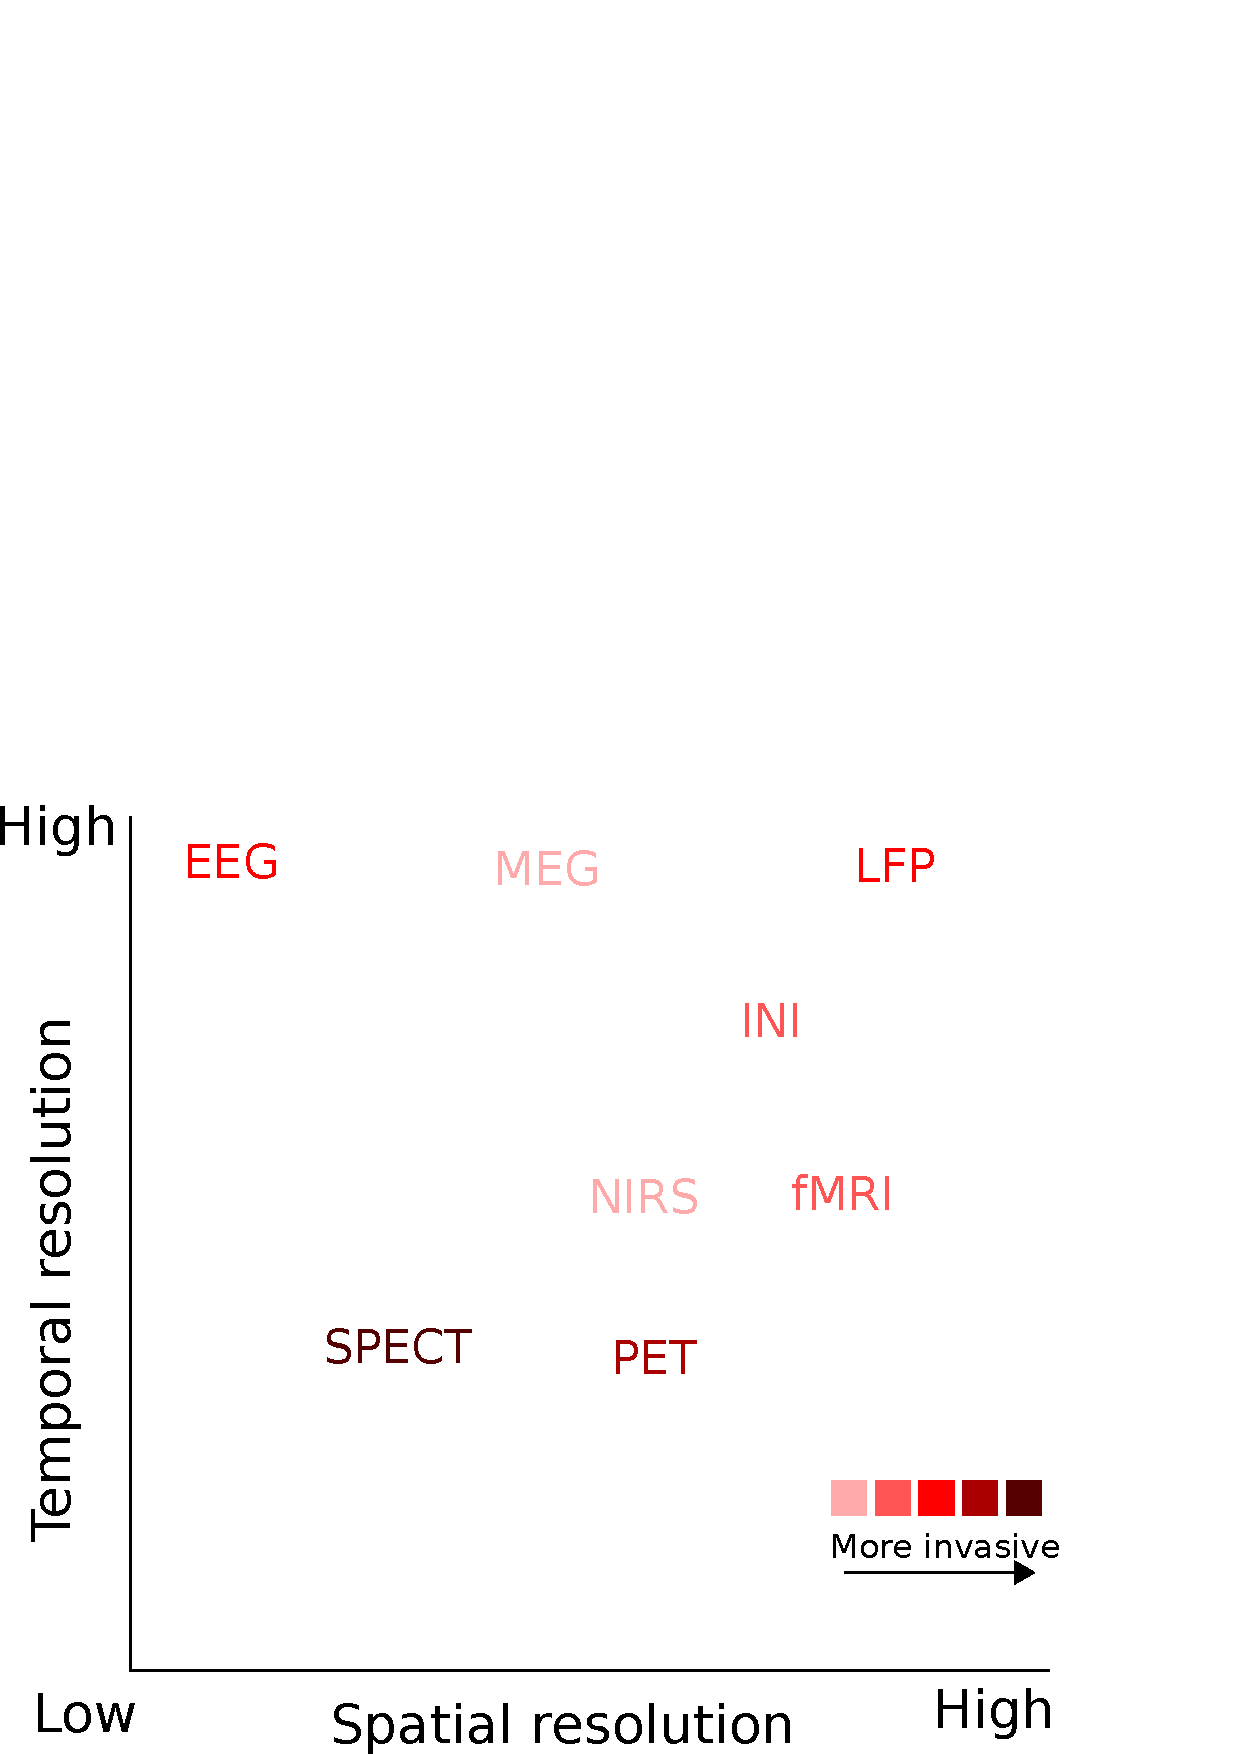
\includegraphics[width=0.5\linewidth]{figures/neuroimaging_methods.pdf}
\end{center}
   \caption[Various neuroimaging methods differ in terms of the information they measure.]{Various neuroimaging methods differ in terms of the information they measure. MEG=magnetoencephalography, EEG=electroencephalography, NIRS=near-infrared spectroscopy, PET=positron emission tomography, SPECT=single photon emission tomography, and INI=Inverse imaging, a method to speed up acquisition of fMRI images, ECoG=Electrocorticography, LFP=Local Field Potential.}
   \label{fig:neuroimaging_methods}
\end{figure}

The study of electrical properties of the biological cells and tissues is known as electrophysiology. 
Biological tissues have electrical properties due to the presence of ions. Just as we can measure voltages in electrical appliances, it is possible also to measure these voltages in living tissues. 
Electrophysiological recording have the advantage of directly measuring the brain activity, as opposed to an indirect measure, which is for example the case in \ac{fMRI}.
Brain imaging techniques are characterized by their temporal and spatial resolution, \textit{i.e.,} the time scale at which it can measure brain activity, and also the accuracy of localizing the source of the activity. Figure~\ref{fig:neuroimaging_methods} summarizes different neuroimaging methods with respect to their temporal and spatial resolution. In the case of \ac{fMRI}, as it measures the blood flow which is a slow response to neural activity, its temporal resolution cannot be high. 

There are a number of methods to measure the electrical potentials in the human body, the most well-known being perhaps \ac{ECG} which is used to measure the electrical activity of the heart. However, in our work, we will focus on only three which are relevant for studying the brain. Each of these methods produces a multivariate time series.

\paragraph{Electroencephalography: } \Ac{EEG} is a portable and non-invasive measurement technique invented in the 1920s that is  used in several contexts such as \acp{BCI}, monitoring and diagnosis, and in cognitive studies. 
In electroencephalography, an array of electrodes on an \ac{EEG} cap is placed on the scalp to measure the voltages with respect to a reference electrode. 
The voltage it measures is not the result of a single neuron but instead a result of the electrical activity of populations of  neurons. It has a high temporal resolution (in the order of \emph{ms}), however the spatial resolution is not so high.

\paragraph{Magnetoencephalography: } Any electric current is associated with magnetic fields as a consequence of Maxwell's theory. 
Therefore, the brain generates tiny magnetic fields which  wrap around the currents according to Maxwell's right hand thumb rule. The field is tiny ($\sim10^{-12}T$) compared to the earth's magnetic field ($\sim10^{-4}T$) and ambient magnetic noise ($\sim10^{-6}T$). Therefore, to measure it, one would need very sensitive electronics and heavy noise cancellation. The measurement itself is done in a magnetically shielded room made of three layers of metals. 
The sensors are superconducting coils which capture the magnetic flux. 
They are immersed in liquid Helium at very low temperatures (around 4 K), so as to lower any loss in signal due to resistance. A typical device contains two types of sensors: gradiometers and magnetometers. While the magnetometer measures the absolute magnitude of magnetic field, the gradiometer measures gradient of the field. \Ac{MEG} has the advantage that the skull does not deteriorate the signal quality as in \ac{EEG}.

\paragraph{\Ac{LFP}}
The Local Field Potential is the electric potential that is recorded in the extracellular space of the brain tissue. In contrast to \ac{EEG}, \ac{LFP} are recorded in depth, from within the cortical tissue and can therefore measure more localized populations of neurons. Small intracerebral electrodes are typically used to measure these potentials as opposed to large surface electrodes used in \ac{EEG}.

\section{Context of the thesis}
This emerges out of the recent movements in reproducibility and data sharing in neuroimaging. It focuses on simplifying data analysis through better educational tools and automated methods to enable reproducible analysis in the age of big data.

\subsection{The reproducibility crisis}
\label{sec:reproducibility_crisis}
Even though thousands of papers are published every year about different aspects of the brain, our understanding of this complex organ has not scaled in proportion. A large part of the reason has been attributed to what is known as the reproducibility crisis~\citep{ioannidis2005most, simmons2011false, button2013power}. %Replication is closely related to the concept of reproducibility which refers to the idea that an experiment produces the same result when performed again under the same conditions. Replication is a stronger condition as it requires similar results or identical conclusion even if there are some minor variations in the experimental procedures. 
Progress in science rests on reproducible experiments. Reproducibility refers to the fact that the findings of an experiment can be regenerated independently if the code, data, and related software was provided. In many fields, however, a large fraction of experiments cannot be reproduced. In psychology, for instance, it was estimated that over half of the papers were not reproducible~\citep{open2015estimating}, and even those which could be reproduced tended to have a weaker effect size compared to the original studies. 

The reasons for unreproducible results can be numerous~\citep{baker20161}, some being: 1) confirmation bias, the tendency to selectively report only experiments that conform to the researcher's pre-existing beliefs, 2) ``p-hacking''~\citep{simmons2011false}, or the tendency to try multiple hypothesis to get a positive result, 3) publication bias or the absence of incentives to publish negative results~\citep{rosenthal1979file}, and 4) pressure to publish. There is now an accepted set of recommendations to address many of these issues: 1) pre-registering research plans to avoid confirmation bias and even report negative results, 2) correct for multiple comparisons, the most conservative method being the Bonferroni correction~\citep{dunn1961multiple}. 

Brain imaging has its own set of issues which can be linked to reproducibility crisis: 

% vul2009puzzlingly
% yendiki2014spurious

\begin{itemize}[noitemsep,partopsep=0pt]
\item \textbf{Power failure:} This is arguably one of the central issues in the reproducibility crisis today and has received by far the most attention. The statistical power of a study refers to the likelihood of discovering an effect of interest, given the sample size. Small sample sizes translate into underpowered studies which means that the chance of a false discovery is high. In order to discover the effect of interest, the study must be appropriately powered.
\item \textbf{Multiple comparison:} This is essentially a manifestation of ``p hacking'' that is a result of of the large number of voxels or time points in neuroimaging. For instance, in the famous dead salmon study~\citep{bennett2009neural}, a significant effect was found even if none was expected simply because the hypothesis testing (comparisons) was done over each voxel.
\item \textbf{Differences in software versions:} Changing software versions can lead to different results. For instance in the case of Freesurfer software, differences in volume were found in the range of $8.8\% \pm 6.6\%$~\citep{gronenschild2012effects}.
\item \textbf{Complex pipelines:} Neuroimaging pipelines involve a number of choices at each processing stage, and there is currently no consensus on how to choose the right pipeline. Often, these methodological choices are not even documented. It is estimated that there are almost as many unique pipelines as there are studies~\citep{Carp2012289}.
\item \textbf{Confounds:} There are several methodological confounds such as head movements~\citep{yendiki2014spurious}, anatomy differences, and changes in breathing rate and depth, which can lead to spurious correlations.
\end{itemize}

In Chapter~\ref{chapter:group_study} of the thesis, we will provide concrete guidelines on how to build processing pipelines for \ac{MEG}/\ac{EEG} data. Our contribution will touch upon the issue of complex pipelines, multiple comparison, and differences in software versions in the context of \ac{MEG}/\ac{EEG}. The issue of power failure can be alleviated through data sharing as I will discuss in the next section.

\subsection{Data sharing}
\label{sec:intro_datasharing}
Power failure is essentially a consequence of small datasets. In today's collaborative and data-driven scientific environment, data sharing is useful not only from the perspective of reproducibility but also to build datasets with large sample sizes. With large datasets, it would be possible to tease apart even subtle effects~\citep{smith2017statistical} that were not possible with smaller datasets. Data sharing is beneficial not just from the perspective of replication but also from an economic perspective. Rather than collect new data for every new hypothesis, researchers can now reuse known data for testing the validity of their hypotheses.

The benefits of data sharing can be traced back to Newton and his theory of gravitation~\citep{pointofview2013}. Before Newton had developed his theory, another English astronomer, John Flamsteed had been appointed by the king to observe the stars and produce accurate charts for navigation in the seas. Over a period of 40 years, Flamsteed created a detailed catalogue that tripled the number of entries in the previously used sky atlas. When the great comet of 1680 appeared in the sky twice in close succession, Flamsteed used his data to postulate that it was not two comets but in fact the same comet which first went towards the sun and then turned away from it. Newton initially opposed this theory, but later changed his mind as he gained access to Flamsteed's unpublished catalogue. The comet had indeed turned out to be an important benchmark for Newton's theory of gravitation.

It is hard to imagine in this day and age that a theory as fundamental as the laws of gravitation could have been data driven. Data sharing is fundamental not only to reproducible science, but also it forms the cornerstone for learning stronger models and benchmarking new algorithms. Consequently, in machine learning, recent breakthroughs have been powered by the increase in data sharing and computation. This includes the recent growth of deep learning~\citep{deng2009imagenet}, Q learning~\citep{watkins1992q, bellemare2013arcade}, natural language processing for language translation~\citep{halevy2009unreasonable}, speech recognition~\citep{paul1992design}, and even the mixture of experts model~\citep{jacobs1991adaptive} for IBM Watson~\citep{ferrucci2010building}. The maxim, ``more data beats a cleverer algorithm''~\citep{domingos2012few} has held up remarkably well across disciplines and over the ages.

Of course, neuroscientists are beginning to realize the importance of sharing data. In recent times, neural data has started being shared through international consortiums~\citep{van2013wu, ollier2005uk}, data repositories~\citep{poldrack2013toward, gorgolewski2015neurovault} and dataset papers in targeted journals. Yet, there is an unaddressed gap in terms of the ideal of data sharing and the practice of data sharing. Neuroimaging experiments are often very complicated, and it is not enough to share simply the data, but also the metadata and information regarding the experimental protocols in a well-structured format. 
In the absence of this information, shared data is not \emph{reusable} in the same way that uncommented and poorly structured, complicated programs are not useful even if shared publicly. 
There is not an accepted consensus in the community on the practices of sharing data and there is a need to establish a standard. 
In Chapter~\ref{chapter:group_study}, we will present a new standard known as the \ac{BIDS}, which is intended to address this gap. 
It is a collaborative effort between software developers and neuroscientists across various laboratories to establish a consensus on the standards and build tools to facilitate adoption of the standard.

\subsection{Automation}
\label{sec:automation}

Back in 2014, Nature published a bold article~\citep{hayden2014automated} which described a vision for the future of science: ``solving the problem of bringing McDonald's-like efficiency to scientists''. This would in turn lead to cheaper, more efficient and reliable research. While it goes on to describe many biology labs which are automating experiments, the benefits of automation in the neuroimaging community are yet to be widely recognized. Automation not only saves time but also makes the research more reproducible, as was noted in a recent guide to improve the transparency and reproducibility of neuroimaging research~\citep{gorgolewski2016practical}. The authors point out that manual work may seem easy at first, if the analysis has to be performed only once. However, this is not always the case as ``quite often in the course of a project, parameters are modified, subjects are changed, and processing steps need to be rerun. This is a situation in which having a set of scripts that can perform all of the processing steps automatically instead of relying on manual interventions can really pay off.'' As large datasets become more common in neuroimaging, automation will indeed become a necessity rather than a luxury.

In neuroimaging, there are in fact several avenues for automation:
\begin{itemize}[noitemsep,nolistsep,nosep]
\item \textbf{Reducing interactivity:} While interactive graphical user interfaces are excellent tools for browsing the data, they fall short when it comes to scaling up the analysis to tens and hundreds of subjects, which is necessary for a sufficiently powered study. 

\item \textbf{Parameter tuning:} Most algorithms, although scripted, still require hyperparameters to be tuned. These hyperparameters could be the number of ICA components to choose or the regularization parameters, and can vary from one subject to the next.
%This could be the number of trials to perform in an experiment, the number of components to select in a \ac{PCA} decomposition, or the regularization parameter in inverse solvers.
\item \textbf{Annotation and labeling:} A large fraction of neuroimaging data that is available is unlabeled or at best weakly labeled. This is because expert annotations are expensive, and cannot be crowdsourced. Automated tools based on unsupervised learning can play a major role in this regard.
\item \textbf{Quality control:} Currently, quality control is performed manually by inspecting the data to spot outliers. While data inspection cannot be overlooked, it can be performed more efficiently through automated documentation of data analysis and log reports such as the Jupyter notebook and the MNE web report~\citep{dengemann2015conc}. At the same time, advanced statistical trend analyses as in the Automated Statistician project~\citep{duvenaud2013structure} can be used for creating summaries.
\end{itemize}

There have been some steps taken in this direction, most notably the Neurosynth platform~\citep{yarkoni2011large} which facilitates large-scale meta analysis. Meta analysis typically combine results from multiple studies, and in this case, it is the brain activation maps from different studies which are combined by using machine learning methods. On the software side, the Freesurfer software package~\citep{dale-fischl-etal:99, fischl-serena-etal:99} provides a \code{recon-all} command that performs cortical segmentation automatically without any human intervention. In MNE, this philosophy is now being adopted starting with automated covariance estimation~\citep{engemann2015automated_new}.

In this thesis, we will consider an algorithm that automatically annotates artifacts in the data~\citep{jas2016automated, jas2017autoreject}. This is a first step that any \ac{MEG}/\ac{EEG} processing pipeline has to go through but it is often done manually. A reason for this is that existing algorithms are not designed to be \emph{transparent}. Since for most scientists, the key to new insights is an artifact-free dataset, they would rather spend extra effort in doing this manually rather than depend on a generic algorithm which is difficult to interpret. %However, this is problematic as it can lead to a selection bias: they might end up rejecting data segments which helps them confirm their hypothesis. 
Merely based on anecdotal reports, this process can take up to a week even for a moderately sized study of 10--20 subjects.

This is what led us to propose \emph{autoreject}, which we describe in Chapter~\ref{chapter:autoreject}. It is an algorithm which can be used to mark bad segments of the data. The key insight is that, often certain sensors in the device are intermittently corrupted rather than continuously. We validate our algorithm against 3 benchmarks on the \ac{HCP} dataset~\citep{larson2013adding} which is manually annotated with bad segments. In the process, our work also represents one of the first attempts at reanalyzing the MEG component of the HCP dataset.

\subsection{Representation learning for data-driven discovery}
\label{sec:representation_learning}
Since the invention of \ac{EEG} in the 1920s, scientists have discovered several different brain oscillation patterns such as alpha waves, K-complexes, and mu rhythms. The oscillations and interactions between them have served as biomarkers for different brain functions and pathologies. Alpha waves have been implicated in attention, K-complexes in sleep, and mu rhythm in motor activity. 

Considering the complexity of the human brain, clearly these waveforms represent only a fraction of the cognitive functions that the brain may perform. As a result of the wealth of data now available through the data sharing movement described in Section~\ref{sec:intro_datasharing}, the future neuroscientist will be able to mine such waveforms from large datasets. Imagine if neuroscientists had at their disposal a tool similar to Google Photos\footnote{\url{https://photos.google.com/}}. In the same way that Google Photos can automatically find faces and group photos, such tools will be able to find prototypical oscillations and cluster the data using them. Clicking on any of these waveforms would retrieve the data associated with them.

\begin{figure}[htb]
\begin{center}
   \includegraphics[width=0.7\linewidth]{figures/schema.pdf}
\end{center}
   \caption[Convolutional sparse coding]{An illustration of how Convolutional sparse coding can be used to automatically mine prototypical waveforms}
   \label{fig:csc_schematic}
\end{figure}

However, photos are inherently different from neural data. First, neural data can be buried in noise and corrupted by high amplitude artifacts. Second, images are labelled owing to crowdsourced data as in the case of  Imagenet~\citep{deng2009imagenet}, but neural data is not. 
Expert annotations in the case of neural data are not easily available.
Finally, it is spatiotemporal data with different dynamics from the 3D world that photos capture. This is where \ac{CSC} can play a role by extracting prototypical features from the data, as shown in Figure~\ref{fig:csc_schematic}. It is an unsupervised algorithm from computer vision, which can learn shift-invariant dictionaries of prototypical waveforms (atoms) from the data using the convolution operations. For a more comprehensive background on \ac{CSC}, the reader may read Section~\ref{sec:background_dict_learning} later in this chapter.

\ac{CSC} algorithms do not approximate the signal using Fourier (or sinusoidal) basis. While this is the conventional technique for extracting signals buried in noise, the approximation can degrade the shape of the signal, which can be a biomarker in many clinical diseases~\citep{cole2017brain}. As an example, even with a large number of sinusoids from the Fourier basis, the edges of a square wave cannot be approximated well. Indeed, the imperfect approximation around such edges is what is often termed as ringing artifacts in signal processing contexts. Of course, transients can be better approximated using wavelets but it is clearly not sufficient for other shapes of data. Rather than fix the basis to be Fourier or wavelet, the \ac{CSC} approach is to learn \emph{both} the basis and the coefficients.

In our work presented in Chapter~\ref{chapter:alphacsc}, we extend conventional \ac{CSC} algorithms for heavy-tailed noise. We reformulate the optimization problem as a \ac{MAP} inference with an alpha-stable distribution to replace the reconstruction loss. Our results show that this kind of algorithm is robust to the presence of artifacts and can be used to uncover temporal structures from neural signals, even those involving nested oscillations.

\clearpage
\section{Brain Imaging Data Structure (BIDS)}

\begin{figure}[htb!]
\begin{center}
   \includegraphics[width=\linewidth]{figures/bids_organization.png}
\end{center}
   \caption[BIDS-MEG data organization scheme.]{BIDS-MEG data organization scheme: Left: a typical default data organization scheme where folders are organized by date of session and contain different runs for a given participant in a study. Right: BIDS-MEG organizes data per study, then participant (subject), followed by modality, then sessions and eventually, runs. Note the sidecar files that are present at all levels of the data hierarchy, and document conveniently the metadata contents.}
   \label{fig:BIDS-MEG-organization}
\end{figure}
From the perspective of reproducibility, data sharing is of paramount importance. Sharing code by itself does not enable reproducibility if the accompanying data is not available, and expensive to acquire. Reanalysis of a dataset is however useful not just from the perspective of reproducibility but also for discovering new effects that were previously overlooked. At the same time, the more data is shared, the larger our sample sizes will be and this will enable us to conduct studies with higher statistical power. Low statistical power, as we discussed in Chapter~\ref{chapter:intro} is one of the main reasons for the reproducibility crisis.

While data sharing in neuroscience is on the rise, the amount of data reuse is still limited. For example, since the release of the Human Connectome Project (HCP)~\citep{larson2013adding} MEG data in 2013, there have been very few instances of reusing this data. At the time of writing this thesis, we had only one or two documented cases~\citep{jas2017autoreject} of reusing the HCP data. Even in these cases, the effort has mostly been limited to reproducing results rather than testing new hypotheses. This clearly represents a gap between the ideal and the practice of data sharing. 

% Clearly, sharing data is not a panacea as the tools, skills and resources to process such large datasets is currently missing in typical laboratories. Perhaps the most important roadblock is standardization of metadata.

Neuroimaging experiments are often complicated involving different  cognitive tasks (auditory, visual, somatosensory \emph{etc.}), different acquisition parameters (sampling frequency, number of sensors and their location, measurement device \emph{etc.}), and population parameters (subject's gender, age \emph{etc.}). All of this metadata is necessary information to successfully reanalyze the data. Unfortunately, historically there has been a lack of consensus amongst different labs and industrial manufacturers as to what constitutes useful metadata. This points to the need for establishing standards. While on a first glance, this may appear to be unnecessary bureaucratic red tape, in fact standards exist in almost all facets of our life. 

Apart from the meta information that is stored with the data, the data itself is stored amongst one of 10--20 different file formats and at different stages of processing. While there have been some efforts previously to standardize data structures~\citep{gibson2009minimum, grewe2011bottom, stoewer2013singlefile, teeters2015neurodata, bigdely2016preparing}, it has not gained wide acceptability. Designing a new standard is tricky as it requires gaining a community consensus. At the same time it must strike the right balance between rigidity for efficiency and flexibility for adapting to future technologies. 

The \ac{BIDS} format~\citep{gorgolewski2016brain} is indeed designed with these considerations in mind. 
The standard involves a hierarchy of folders to describe the imaging technology used, the name of the subject, and the date of the experiment. 
At each level of hierarchy, files are accompanied by sidecar \code{json} files describing the metadata. 
A \code{json} file is an easy to parse text file that contains key and value pairs, so that it has the advantage of being machine and human readable at the same time. 
These files follow an \emph{inheritance principle}, that is, a field described in a \code{json} file in a higher level of the hierarchy will be automatically propagated downstream. 
The main BIDS specification is accompanied by extension specifications which describe specific aspects to describe different modalities.
At the same time, the standard does not exist in isolation.
The \ac{BIDS} consortium is also providing a growing ecosystem of tools to convert datasets into \ac{BIDS} compatible format as well as to validate data to conform to the standard. 

In the present work, we present a significant extension of \ac{BIDS} to support the specific aspects of \ac{MEG} data. \Ac{MEG}, as we know from Chapter~\ref{chapter:intro}, provides direct measurement of brain activity with millisecond temporal resolution and unique source imaging capabilities. So far, \ac{BIDS} has provided a solution to structure the organization of \ac{MRI} data. Despite the lack of standard data format for \ac{MEG}, BIDS-MEG is a principled solution to store, organize and share the typically-large data volumes produced. It builds on \ac{BIDS} for \ac{MRI}, and therefore readily yields a multimodal data organization by construction. This is particularly valuable for the anatomical and functional registration of \ac{MEG} source imaging with \ac{MRI}. With BIDS-MEG and a growing range of software adopting the standard, the \ac{MEG} community has a solution to minimize curation overheads, reduce data handling errors and optimize usage of computational resources for data analysis. The standard also includes well-defined metadata to facilitate future data harmonization and sharing efforts, and extensions to other electrophysiological data modalities.

\clearpage
\section{A reproducible M/EEG group study}

\begin{figure}[t]
  \centering
  \includegraphics[width=0.7\linewidth]{figures/grand_average_highpass-NoneHz.pdf}\\
  \includegraphics[width=0.7\linewidth]{figures/grand_average_highpass-1Hz.pdf}
\caption[Grand averaged evoked response across 16 subjects.]{Grand averaged evoked response across 16 subjects for channel EEG065.
(A) No highpass filter. (B) Highpass filtered at 1.0 Hz. Note that, similar to (A), the results reported by \cite{wakeman2015multi} (dashed line at 800 ms indicates where their plot stopped) show large drifts, but these return to near-baseline levels toward the end of a sufficiently long interval (here, 2.9 seconds) even without applying a highpass filter.}
\label{fig:grand_average}
\end{figure}  

In the previous chapter, we discussed how data sharing can be facilitated using the \ac{BIDS} for \ac{MEG}. This is taking us one step closer to the goal of reproducibility. However, reproducibility is not achieved by merely sharing more data with the hope that this will solve all problems. As noted in \citet{baker20161}, one of the best solutions to foster reproducible science is not a technical one, but an educational one. This is of course true for statistics, where there is an urgent need to clarify and educate researchers about the statistical tools required in neuroscience. But it is now increasingly important also for academic software.

In recent years, free academic toolboxes have gained increasing prominence in \ac{MEG} analysis as a means to disseminate cutting edge methods, share best practices between different research groups and pool resources for developing essential tools for the \ac{MEG} community. Teaching events are regularly held around the world where the basics of each toolbox are explained by its  developers and experienced power users. There are however, knowledge gaps that need to be addressed. First, most teaching examples only show analysis of a single ‘typical best’ subject whereas most real MEG studies involve analysis of group data. It is then left to the researchers in the field to figure out for themselves how to make the transition and obtain significant group results. Secondly, we are not familiar with any examples of fully analyzing the same group dataset with different academic toolboxes to assess the degree of agreement in scientific conclusions and compare strengths and weaknesses of various analysis methods and their independent implementations.

To address this very issue, a workshop was organised by the lead developers of six most popular free academic MEG toolboxes at Biomag 2017. This work is a follow up to the workshop, which presents the contribution of the MNE software team, and will be published in \emph{Frontiers in Neuroscience, section Brain Imaging Methods}. This study presents the results obtained by the reanalysis of an open dataset from \citet{wakeman2015multi} using the MNE software package. The analysis covers preprocessing steps, quality assurance, sensor-space analysis of evoked responses, source localization, and statistics in both sensor and source space. Results with possible alternative strategies are presented and discussed at different stages such as the use of high-pass filtering versus baseline correction, tSSS versus \ac{SSS}, the use of a minimum norm inverse versus \ac{LCMV} beamformer, and the use of univariate or multivariate statistics. This aims to provide a comparative study of different stages of \ac{MEG}/\ac{EEG} analysis pipeline on the same dataset, with open access to all of the scripts necessary to reproduce this analysis.

\clearpage

\section{Automated artifact rejection for M/EEG}

\begin{figure}[t]
	\centering
	\includegraphics[width=0.8\linewidth]{figures/figure1.pdf}
    \caption[Cross-validation error as a function of peak-to-peak rejection threshold on one EEG dataset.]{Cross-validation error as a function of peak-to-peak rejection threshold on one EEG dataset. The root mean squared error (RMSE) between the mean of the training set (after removing the trials marked as bad) and the median of the validation set was used as the cross-validation metric (Section~\ref{sec:auto_global}). The two insets show the average of the trials as ``butterfly plots" (each curve representing one sensor) for very low and high thresholds. For low thresholds, the RMSE is high because most of the trials are rejected (underfit). At high thresholds, the model does not drop any trials (overfit). The optimal data-driven threshold (\emph{autoreject, global}) with minimum RMSE is somewhere in between. It closely matches the human threshold.}
    \label{fig:cross_val}
\end{figure}

In the last chapter, we discussed the reproducibility challenges when performing group studies in \ac{MEG} and \ac{EEG}. One way to improve reproducibility is automation, and we briefly touched upon an algorithm for automating detection of bad data segments, known as \emph{autoreject}.

%copy pasted abstract below
In this chapter, we will present this algorithm which rejects and repairs bad trials in \ac{MEG} and \ac{EEG} signals. Annotating bad segments in the data is perhaps one of the most time consuming aspects of data processing in electrophysiology. Currently, it is either done manually, or using automated black-box algorithms. The manual approach is often subjective with often no clear consensus on what constitutes a corrupted data segment. Therefore, reanalysis is not only manually demanding but can also lead to problems in reproducibility. On the other hand, the automated methods are controlled by parameters that are not straightforward to tune. In the case of failure, it is not always obvious what caused the method to fail and how it can be corrected. As a result, one is left with no choice but to exclude the data from further analysis.

This led us to develop a method based on design choices motivated by ease of interpretation and diagnosis. The method we propose capitalizes on cross-validation in conjunction with a robust evaluation metric to estimate the optimal peak-to-peak threshold--a quantity commonly used for identifying bad trials in \ac{MEG}/\ac{EEG}. This approach is then extended to a more sophisticated algorithm which estimates this threshold for each sensor yielding trial-wise bad sensors. Depending on the number of bad sensors, the trial is then repaired by interpolation or by excluding it from subsequent analysis. For efficiency reasons, we use Bayesian optimization which is a well-known technique for hyperparameter optimization. All steps of the algorithm are fully automated thus lending itself to the name \emph{autoreject}. Crucially, the algorithm is even able to deal with sensors that are locally corrupted, which is quite often the case for \ac{EEG} data.

In order to assess the practical significance of the algorithm, we conducted extensive validation and comparisons with state-of-the-art methods on four public datasets containing \ac{MEG} and \ac{EEG} recordings from more than 200 subjects. The comparisons include purely qualitative efforts as well as quantitatively benchmarking against human supervised and semi-automated preprocessing pipelines. The algorithm allowed us to automate the preprocessing of \ac{MEG} data from the \ac{HCP} going up to the computation of the evoked responses. The automated nature of our method minimizes the burden of human inspection, hence supporting scalability and reliability demanded by data analysis in modern neuroscience.

\clearpage
\section{Temporal representation learning}

So far, we studied automation in neuroimaging with the objective of enabling scalable data analysis and reproducibility. While  reproducibility and large-scale data analysis allow us to consolidate upon existing studies, \emph{per se} they are not tools to uncover new and interesting phenomena. In this chapter, we will explore this dimension of automation using what is known as \emph{representation learning}.

Representations are the building blocks of signal processing. It is quite easy to convince ourselves of this fact, if we simply use a Fast Fourier Transform (FFT) to filter data. When we are using an FFT, we are in effect, decomposing the signal into a sum of sinusoids of varying frequencies. If we are interested in a time-frequency analysis, a common choice of representation for neurosience signals consists in using Morlet wavelets.

Traditionally, the choice of representation has been mainly driven by analytical concern and ease of mathematical manipulation. However, the recent surge of deep learning has ignited an interest in data-driven representations. It is because good representations  that compactly capture the properties of the data are essential for efficient and accurate learning systems. In computer vision, for instance, handcrafted features such as SIFT~\citep{lowe1999object} and GIST descriptors~\citep{oliva2001modeling}, Deformable Parts Model (DPM)~\citep{felzenszwalb2010object}, Histogram of Oriented Gradient (HOG)~\citep{dalal2005histograms} \emph{etc.} had been the norm, before it was realized that unsupervised learning and autoencoders performed much better.

Today, unsupervised learning is used as a first step for a supervised learning task in computer vision. Representation learning, by itself, is perhaps not as interesting, except for diagnostic visualizations in deep learning~\citep{zeiler2014visualizing}. Despite this, there has always been an interest in understanding representations in the human brain (visual system particularly), as it was thought that this would help us build better learning systems. One of the pioneers in this area of research is Bruno Olshausen, whose work on dictionary learning~\citep{olshausen1996emergence} demonstrated that Gabor patches are indeed fundamental to natural images, similar to the ones that Hubel and Wiesel~\citep{hubel1962receptive, marcelja1980mathematical} found in the cat visual cortex, and to what is used in GIST features. Barring this line of studies, the learned representation itself is not considered as meaningful as performance metrics like the prediction score or reconstruction loss. However, in the case of neural signals, we realized that this is not the case and the fidelity of the representation is in itself interesting. Indeed, the shape of the signal is a crucial biomarker in many clinical applications for neuroscience~\citep{cole2017brain}. 

A parallel development in the field of neuroimaging has been the rise in interest for learning prototypical shapes which are shift invariant~\citep{jost2006motif, barthelemy2013multivariate, brockmeier2016learning, hitziger2017adaptive}. It is motivated by the fact that existing approximations using the Fourier basis often distorts the signal. There is, for example, a debate regarding the type of filters that should be used (See Section~\ref{sec:group_study_temporal_filtering} and \cite{widmann2015digital,parks1987digital,ifeachor2002digital, gotz-etal:15}). 
Even though some success has been reported
with these algorithms in neuroimaging, they are limited in applicability due to their heuristic nature.
Remarkably, there has been so far very little cross-pollination of ideas between the computer vision and neuroimaging communities on these sparse coding aspects. 
Our work is an attempt to bridge this gap. 
We propose a model which builds upon existing shift-invariant sparse coding models to be able to handle heavy-tailed noise and artifacts. It assumes positivity of the coefficients to account for the fact that an atom does not change polarity over time. 

Our model is a novel probabilistic \ac{CSC} model for learning shift-invariant atoms from unprocessed neural time series data containing
potentially severe artifacts.
In the core of our model, which we call $\alpha$CSC, lies a family of heavy-tailed
distributions called $\alpha$-stable distributions. We develop a novel, computationally efficient Monte Carlo
expectation-maximization algorithm for inference. The maximization step boils down to a weighted
\ac{CSC} problem, for which we develop a computationally efficient optimization algorithm.

In our work, we rigorously evaluate the computational efficiency of our algorithm against the competing benchmarks. Because the \ac{CSC} problem is non-convex, the optimization procedure involves nested loops and theoretical analysis often falls short in dealing with the complexity of non-convex functions. 
The optimization procedure is nested as the problem is convex when one of the variables is fixed: the atoms or the activations. The outer loop alternates between these two variables while the inner loop learns them when the other is fixed. An experimental approach, while challenging, is not completely out of reach. The final result depends on the initialization, and therefore algorithms can be compared only if they are tested for many different random seeds and their results averaged. Our qualitative analysis also goes beyond the narrative of verifying the existence of known waveforms to uncovering more complex structures in the data.

Our results
show that the proposed algorithm achieves state-of-the-art convergence speeds. Besides, $\alpha$CSC is
significantly more robust to artifacts when compared to three competing algorithms: it can extract
spike bursts, oscillations, and even reveal more subtle phenomena such as cross-frequency coupling
when applied to noisy neural time series.

\begin{figure}[t]
    \centering
     \subfigure[$K=10$, $L=32$.]{
     \includegraphics[width=0.5\linewidth]{figures/relative_10_32.pdf}} \\
     \subfigure[Time to reach a relative precision of 0.01.]{
     \includegraphics[width=\textwidth]{figures/bar_plot.pdf}}
    \caption[Comparison of state-of-the-art methods with our approach.]{Comparison of state-of-the-art methods with our approach. (a)~Convergence plot with the objective function relative to the obtained minimum, as a function of computational time. (b)~Time taken to reach a relative precision of $10^{-2}$, for different settings of $K$ and $L$.  }
    \label{fig:convergence}
\end{figure}

\begin{figure}[b]
    \centering
             \subfigure[LFP spike data from \cite{hitziger2017adaptive}]{
             \includegraphics[height=3cm]{figures/spike_atomsa.pdf}
             \label{fig:spikedata}}
             \subfigure[Estimated atoms]{
             \includegraphics[height=2.9cm]{figures/spike_atomsb.pdf}
             \label{fig:spikeatoms}}

            \caption[Atoms learnt by $\alpha$CSC on LFP data containing epileptiform spikes with $\alpha=2$.]{Atoms learnt by $\alpha$CSC on LFP data containing epileptiform spikes with $\alpha=2$.}
\end{figure}

Methods research in neuroimaging is a marriage between computer science and neuroscience. It is a collaboration between two complementary disciplines -- the aim is to bring to the table computation tools which can help scientists make new discoveries. Certain aspects of this interdisciplinary subfield is of course to incrementally develop existing tools: for example, those that can help achieve a better prediction score, or a better localization accuracy in estimating neural sources. However, an orthogonal but equally important aspect of methods research is to develop tools which allow fundamentally new ways to interact with the data. This thesis is an attempt to advance this goal by developing tools for automated analysis in electrophysiology.

It has now become evident to us that in order to achieve the goal of reproducible research, large public datasets are the key and automated methods to analyze them are indispensable. While every neuroscientist's ambition is to generate new insights and push the frontiers of our knowledge of the brain, this is often not possible due to the weak effect sizes which cannot be uncovered in small datasets. When the null hypothesis cannot be rejected, it is a common practice to start fishing for significant results by testing multiple hypotheses and reporting the most favourable ones. This has resulted in a body of literature where a large fraction of the results lie on shaky grounds. 

In this thesis, we developed a new specification known as the \ac{BIDS}, which facilitates data sharing between neuroscientists by promoting common standards for storing measurement related metadata. We also provided an overview of the challenges in reproducible data analysis with respect to \ac{MEG}/\ac{EEG} data. As contributors to the MNE software package, we felt particularly well positioned to address  the software related challenges: complex pipelines, software versions, random initialization \emph{etc.,} and standardized recommendations for each stage of these pipelines. We did this by reanalyzing a group study on Faces dataset~\citep{wakeman2015multi}. To ensure reproducible results, the entire analysis was scripted and the plots generated automatically using the \code{sphinx\_gallery} package\footnote{https://sphinx-gallery.github.io}.

In order to even further push the goal of reproducibility via automation, we developed two new methods for analyzing electrophysiological data. The first method, called \emph{autoreject}, aims to streamline the removal of data segments containing artifacts which is a basic preprocessing step in almost every analysis chain. We develop an efficient method which uses a parameter search method known as Bayesian optimization. Our approach was able to facilitate re-analysis of the \ac{HCP} data for benchmarking. Our second method, known as \emph{alphacsc} enables mining neural time series for new oscillatory structures. Not only that, it is a tool to estimate more accurate waveform shapes than what is possible using traditional Fourier analysis. We demonstrated in our work that it was able to discover nested oscillations from the data.

These technologies can still be considered to be in their infancy in many respects. Just as source localization methods in \ac{MEG}/\ac{EEG} have evolved from dipole-based models to distributed methods to more sophisticated models implementing structured sparsity, these new methods are likely to undergo an evolutionary process of incremental improvements. If we consider the example of \ac{CSC}, our model based on alpha-stable distributions extended the computer vision models to be able to handle heavy-tailed distributions that is characteristic in neural data. Obviously, this is not the end of the road. Tuning hyperparameters in \ac{CSC} models is still notoriously difficult, but it is not impossible if there is an supervised task at the end of the pipeline. Multiscale dictionaries might be critical for brain signals considering that the oscillations can have varying support. As the problem is non-convex, smarter initialization strategies such as those based on \ac{MCMC} could lead to more accurate estimates~\citep{bachem2016fast}. It will also soon be necessary to build streaming \ac{CSC} algorithms based on stochastic approximations to deal with larger datasets.

Unlike computer vision or natural language processing, high-risk industries such as healthcare require transparent algorithms. It is no longer sufficient to be able to merely achieve higher prediction accuracy.
% In fact, a large fraction of neuroimaging data, even that which is available publicly, is unlabeled or at best weakly labeled.
In our work on \emph{autoreject} and \emph{alphacsc}, we leverage such public data to develop algorithms which are easy to interpret and diagnose. \emph{Autoreject} identifies the data segments to be removed based on a single parameter which is easy to understand and is automatically tuned. In the same way, \emph{alphacsc} mines the prototypical waveforms directly so as to replace indirect measures for unearthing phenomena of interest.

In this thesis, I outlined a strategy for reproducible research in the future: public datasets with large sample sizes and automation. However, the focus of some of my work was limited to automation on the scale of single subjects. Even though this does enable us to analyse large datasets, it can be sometimes limiting as it does not allow us to pool data across subjects so as to discover more subtle effects. As we enter an era of fast-paced science, such data-driven tools will become indispensable. While a lot of methods research has been focussed on improving the signal-to-noise ratio in each dataset, this may turn out to be not as important when dealing with larger datasets. Looking ahead, we will increasingly prefer large datasets which are not perfectly denoised rather than a smaller perfectly denoised dataset. New tools will need to be developed in order to enable clinicians to rapidly probe the brain so as to identify signals and structures of interest, quantify uncertainties along with the accuracy scores, perform quality control, and interactively visualize their data.
